\section{Wyprzedzające pobranie danych}

Wyprzedzające pobranie danych potraktowaliśmy jako swego rodzaju eksperyment. Nasze obawy związane z optymlizacją kody okazały się być uzasadnione. W celu realizacji problemu dodaliśmy zmienną $tmp$, na której nie były realizowane żadne operacje. Eksperyment podzieliliśmy na dwie części.

\subsection{Klasyczne podejście}

Początkowo spodziewaliśmy się, że kompilator usunie nic nie robiące przepisanie. Po przejrzeniu instrukcji Assemblera okazało się, że jest inaczej.

\begin{figure}[!ht]
\centering
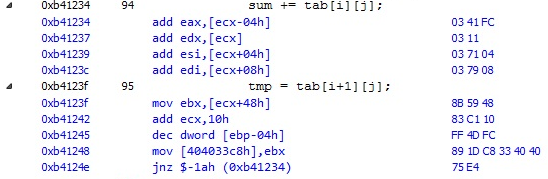
\includegraphics[width=0.9\textwidth]{pf.png}
\caption{Instrukcja przypisania do zmiennej $tmp$}
\end{figure}

\begin{table}[H]
\centering
\begin{tabular}{|l|c|}
\hline
Algorytm & Czas [ms] \\ \hline
$sum\_ij$ & 253 \\ \hline
$sum\_pf$ & 225 \\ \hline
\end{tabular}
\caption{Czasy algorytmów kluczowych dla wyprzedzającego pobrania}
\end{table}

Przyspieszenie związane z wyprzedzającym pobraniem danych okazało się jednak być bardzo nieznaczne.

\subsection{Zastosowanie kwalifikatora $volatile$}

$volatile$ w C++ jest kwalifikatorem typu informującym kompilator, ze wartość zmiennej może się zmienić bez jego wiedzy i kontroli i że w związku z tym kompilator powinien zrezygnować z agresywnej optymalizacji i przy każdym odwołaniu do tej zmiennej wczytać nową wartość z komórki pamięci.\newline

Kod odpowiedzialny za inicjalizację zmiennej $tmp$ prezentował się następująco:

\begin{lstlisting}[caption=Definicja $tmp$ z użyciem volatile., captionpos=none]
volatile int tmp;
\end{lstlisting}

Zastosowanie wyżej wymienionego kwalifikatora spowodowało zgodnie z oczekiwaniami pogorszenie czasu przetwarzania.



